%%%%%%%%%%%%%%%%%%%%%%%%%%%%%%%%%%%%%%%%%%%%%%%%%%%%%%%%%%%%%%%
%
% Welcome to Overleaf --- just edit your LaTeX on the left,
% and we'll compile it for you on the right. If you open the
% 'Share' menu, you can invite other users to edit at the same
% time. See www.overleaf.com/learn for more info. Enjoy!
%
%%%%%%%%%%%%%%%%%%%%%%%%%%%%%%%%%%%%%%%%%%%%%%%%%%%%%%%%%%%%%%%


% Inbuilt themes in beamer
\documentclass{beamer}
\usepackage{setspace}
\usepackage{gensymb}
\singlespacing
\usepackage{amsmath}
\usepackage{bm}
\usepackage{cite}
\usepackage{cases}
\usepackage{subfig}
\usepackage{longtable}
\usepackage{multirow}
\usepackage{verbatim}
\usepackage{hyperref}
\usepackage{listings}
\usepackage{color}    
\usepackage{array}    
\usepackage{longtable}
\usepackage{calc}     
\usepackage{multirow} 
\usepackage{hhline}   
\usepackage{ifthen}   
\DeclareMathOperator*{\Res}{Res}

% correct bad hyphenation here
\hyphenation{op-tical net-works semi-conduc-tor}
\def\inputGnumericTable{}                                 %%

\lstset{
%language=C,
frame=single, 
breaklines=true,
columns=fullflexible
}
%\lstset{
%language=tex,
%frame=single, 
%breaklines=true
%}
\hypersetup{
    colorlinks=true,
    linkcolor=black,
    urlcolor=blue,
}
\usetheme{CambridgeUS}

\DeclareMathOperator*{\argmax}{arg\,max}
\DeclareMathOperator*{\argmin}{arg\,min}
\newtheorem{proposition}{Proposition}[section]
\newcommand{\BEQA}{\begin{eqnarray}}
\newcommand{\EEQA}{\end{eqnarray}}
\newcommand{\define}{\stackrel{\triangle}{=}}
\bibliographystyle{IEEEtran}
\providecommand{\mbf}{\mathbf}
\providecommand{\pr}[1]{\ensuremath{\Pr\left(#1\right)}}
\providecommand{\qfunc}[1]{\ensuremath{Q\left(#1\right)}}
\providecommand{\sbrak}[1]{\ensuremath{{}\left[#1\right]}}
\providecommand{\lsbrak}[1]{\ensuremath{{}\left[#1\right.}}
\providecommand{\rsbrak}[1]{\ensuremath{{}\left.#1\right]}}
\providecommand{\brak}[1]{\ensuremath{\left(#1\right)}}
\providecommand{\lbrak}[1]{\ensuremath{\left(#1\right.}}
\providecommand{\rbrak}[1]{\ensuremath{\left.#1\right)}}
\providecommand{\cbrak}[1]{\ensuremath{\left\{#1\right\}}}
\providecommand{\lcbrak}[1]{\ensuremath{\left\{#1\right.}}
\providecommand{\rcbrak}[1]{\ensuremath{\left.#1\right\}}}
\theoremstyle{remark}
\newtheorem{rem}{Remark}
\newcommand{\sgn}{\mathop{\mathrm{sgn}}}
\providecommand{\abs}[1]{\left\vert#1\right\vert}
\providecommand{\res}[1]{\Res\displaylimits_{#1}} 
\providecommand{\norm}[1]{\left\lVert#1\right\rVert}
\providecommand{\mtx}[1]{\mathbf{#1}}
\providecommand{\mean}[1]{\mathbb{E}\left[ #1 \right]}   
\providecommand{\fourier}{\overset{\mathcal{F}}{ \rightleftharpoons}}
\providecommand{\system}[1]{\overset{\mathcal{#1}}{ \longleftrightarrow}}
\newcommand{\cosec}{\,\text{cosec}\,}
\providecommand{\dec}[2]{\ensuremath{\overset{#1}{\underset{#2}{\gtrless}}}}
\newcommand{\myvec}[1]{\ensuremath{\begin{pmatrix}#1\end{pmatrix}}}
\newcommand{\mydet}[1]{\ensuremath{\begin{vmatrix}#1\end{vmatrix}}}
\renewcommand{\vec}[1]{\mathbf{\boldsymbol{#1}}}
% Theme choice:
\newcounter{saveenumi}
\newcommand{\seti}{\setcounter{saveenumi}{\value{enumi}}}
\newcommand{\conti}{\setcounter{enumi}{\value{saveenumi}}}

\resetcounteronoverlays{saveenumi}
% Title page details: 
\title[ESP32 Weather Station]{Simple Weather Station Using ESP32} 
\author{Gautam Singh}
\begin{document}

% Title page frame
\begin{frame}
    \titlepage 
\end{frame}

% Remove logo from the next slides
\logo{}

% Outline frame
\begin{frame}{Outline}
    \tableofcontents
\end{frame}

% Lists frame
\section{Introduction}
\begin{frame}{Aim}
    Use machine learning to build a simple weather station  with a web interface
    using a PT-100 and ESP32.
\end{frame}

\section{Resources}
\begin{frame}{Hardware}
    \begin{enumerate}
        \item ESP32 microcontroller with Type-B USB cable
        \item PT-100 RTD
        \item Breadboard and Jumper Wires
        \item Android phone
        \item (Optional) USB 2.0/3.0 Hub
    \end{enumerate}
\end{frame}

\begin{frame}[label=software]{Software}
Relevant platformio codes can be found 
\href{https://github.com/goats-9/ee2802-assignments/tree/main/pt100/esp32/codes/esp32}{here}.
\begin{enumerate}
    \item In this directory, type \texttt{pio run} to generate the firmware to
    flash to the ESP32.
    \item Using ArduinoDroid, flash it to the ESP32 from your Android phone.
    \item Run the server by typing \texttt{flask run --host=<YOUR HOST IP>}.
\end{enumerate}
A more detailed manual is present \href{https://github.com/goats-9/ee2802-assignments/tree/main/pt100/esp32/main.pdf}{here}.
\end{frame}

\begin{frame}{Setup for Experiment}
    \begin{figure}[!ht]
        \centering
        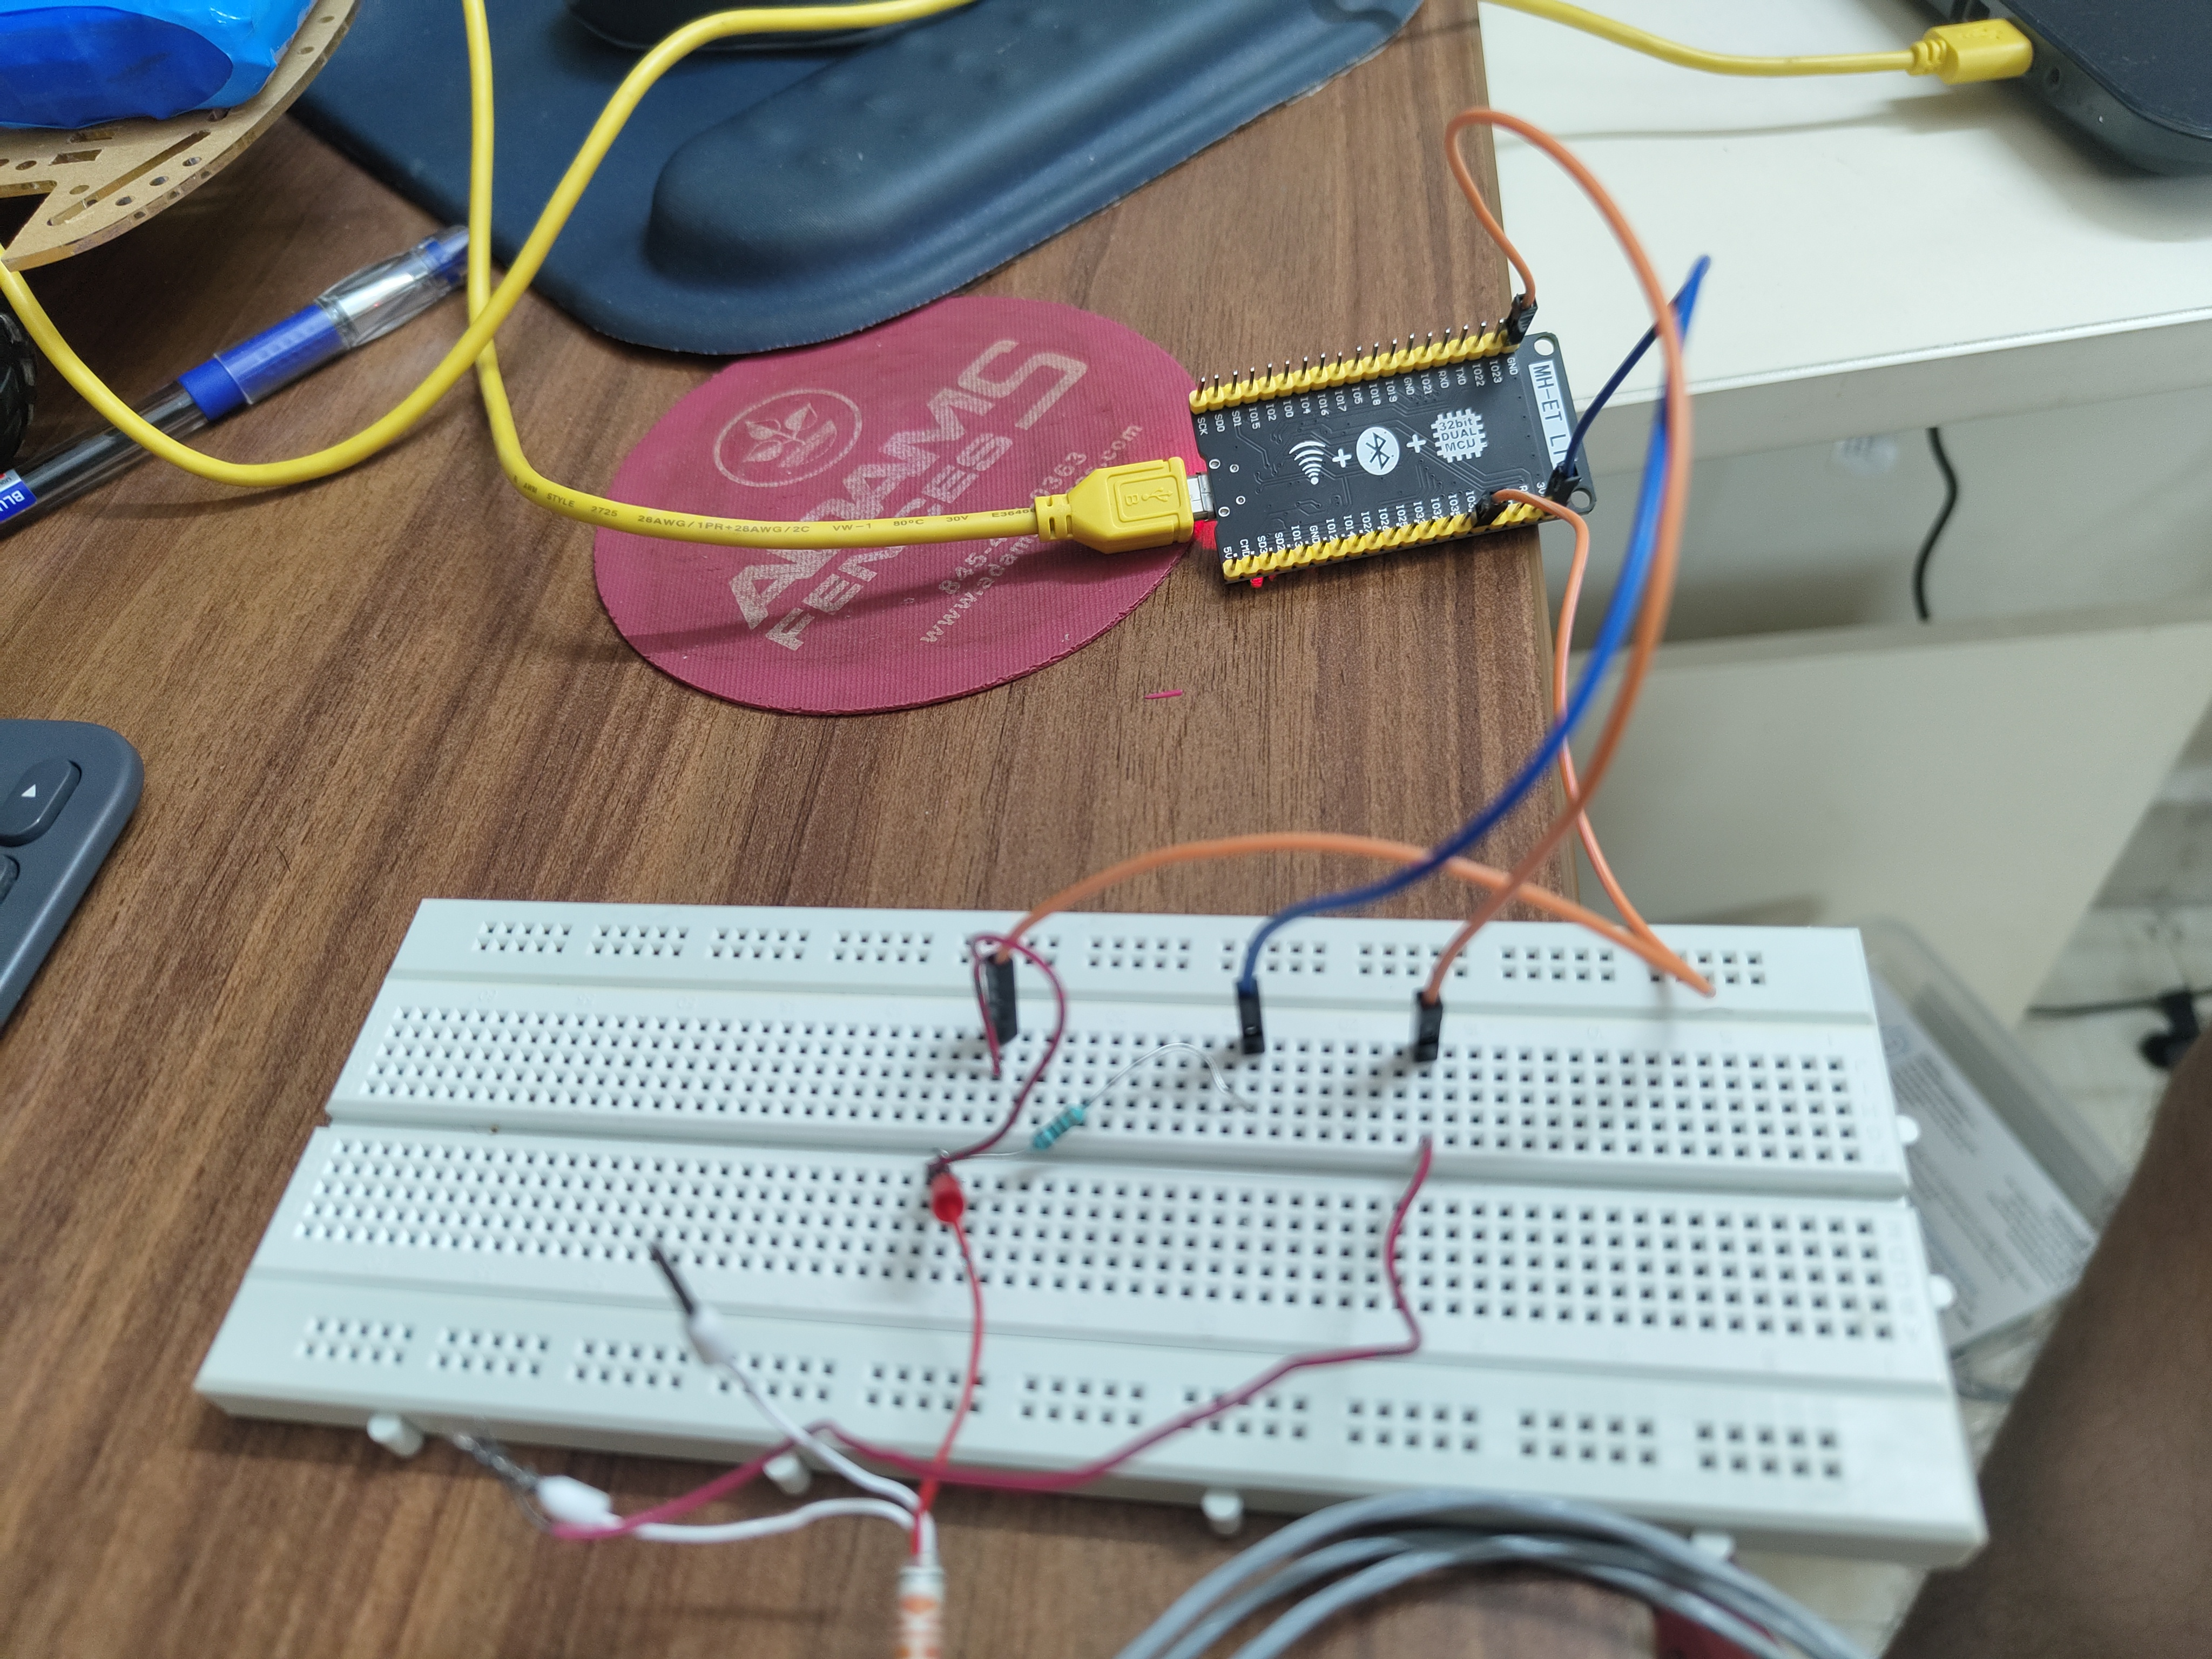
\includegraphics[width=0.6\columnwidth]{figs/esp32.jpg}
        \caption{Setup for Weather Station.}
        \label{fig:setup}
    \end{figure}
\end{frame}

\section{Working}
\begin{frame}{Underlying Principles}
    \begin{enumerate}
        \item The PT-100 is a resistance temperature detector (RTD),
        \pause
        \item It is governed by the Callendar van Dusen Equation
        \begin{align}
            V(T) &= V(0)\brak{1 + AT + BT^2} \\
                 &= V(0)\myvec{1&A&B}\myvec{1\\T\\T^2}
        \end{align}
        \pause
        \item We can use the least squares method to find the coefficients.
    \end{enumerate}
\end{frame}

\section{Demonstration}
\begin{frame}
    \begin{center}
        \Huge In-Class Demonstration
    \end{center}
\end{frame}

\begin{frame}
    \begin{center}
        \Huge Thank You!
    \end{center}
\end{frame}
\end{document}
